\documentclass[a4paper,12pt]{article}
\usepackage[T1]{fontenc}
\usepackage[utf8]{inputenc}
\usepackage{polski}
\usepackage{color}
\usepackage{graphicx}
\usepackage{amsmath}
\usepackage{amssymb}
\usepackage{hyperref}
\usepackage{float}
\usepackage{listings}
\usepackage[backend=biber]{biblatex}

\addbibresource{bibliografia.bib}

\lstset{
  basicstyle=\ttfamily,
  columns=flexible,
  keepspaces=true,
  literate={ą}{{\k{a}}}1
           {ć}{{\'{c}}}1
           {ę}{{\k{e}}}1
           {ł}{{\l{}}}1
           {ń}{{\'{n}}}1
           {ó}{{\'{o}}}1
           {ś}{{\'{s}}}1
           {ź}{{\'{z}}}1
           {ż}{{\.{z}}}1
           {Ą}{{\k{A}}}1
           {Ć}{{\'{C}}}1
           {Ę}{{\k{E}}}1
           {Ł}{{\L{}}}1
           {Ń}{{\'{N}}}1
           {Ó}{{\'{O}}}1
           {Ś}{{\'{S}}}1
           {Ź}{{\'{Z}}}1
           {Ż}{{\.{Z}}}1
}

\title{Zadanie - wykład 3}
\author{Mikołaj Kubś, 272662}
\date{\today}

\begin{document}

\maketitle

\begin{figure}[H]
  \centering
  
\includegraphics[width=1\textwidth]{images/task1.png}
  \caption{Opis zadań 1-3}
\end{figure}

\begin{figure}[H]
  \centering
  
\includegraphics[width=1\textwidth]{images/task2.png}
  \caption{Opis zadań 4-6}
\end{figure}

\section{Kod kwerend 1-3}

\subsubsection{1.}

Jaka była łączna suma transakcji (SalesOrderHeader.SubTotal) w poszczególnych latach dla kolejnych dni tygodnia?

\begin{lstlisting}[
  language=SQL,
  showspaces=false,
  basicstyle=\ttfamily,
  numbers=left,
  numberstyle=\tiny,
  commentstyle=\color{green},
  tabsize=2
  ]
SET DATEFIRST 1;
SET LANGUAGE Polish;

SELECT 
  SUM(SubTotal) AS "Suma",
  DATENAME(DW, OrderDate) AS "Dzień tygodnia",
  DATEPART(YEAR, OrderDate) AS "Rok"
FROM Sales.SalesOrderHeader
GROUP BY 
  DATENAME(DW, OrderDate), 
  DATEPART(YEAR, OrderDate), 
  DATEPART(DW, OrderDate)
ORDER BY DATEPART(YEAR, OrderDate), DATEPART(DW, OrderDate)
\end{lstlisting}

\begin{figure}[H]
  \centering
  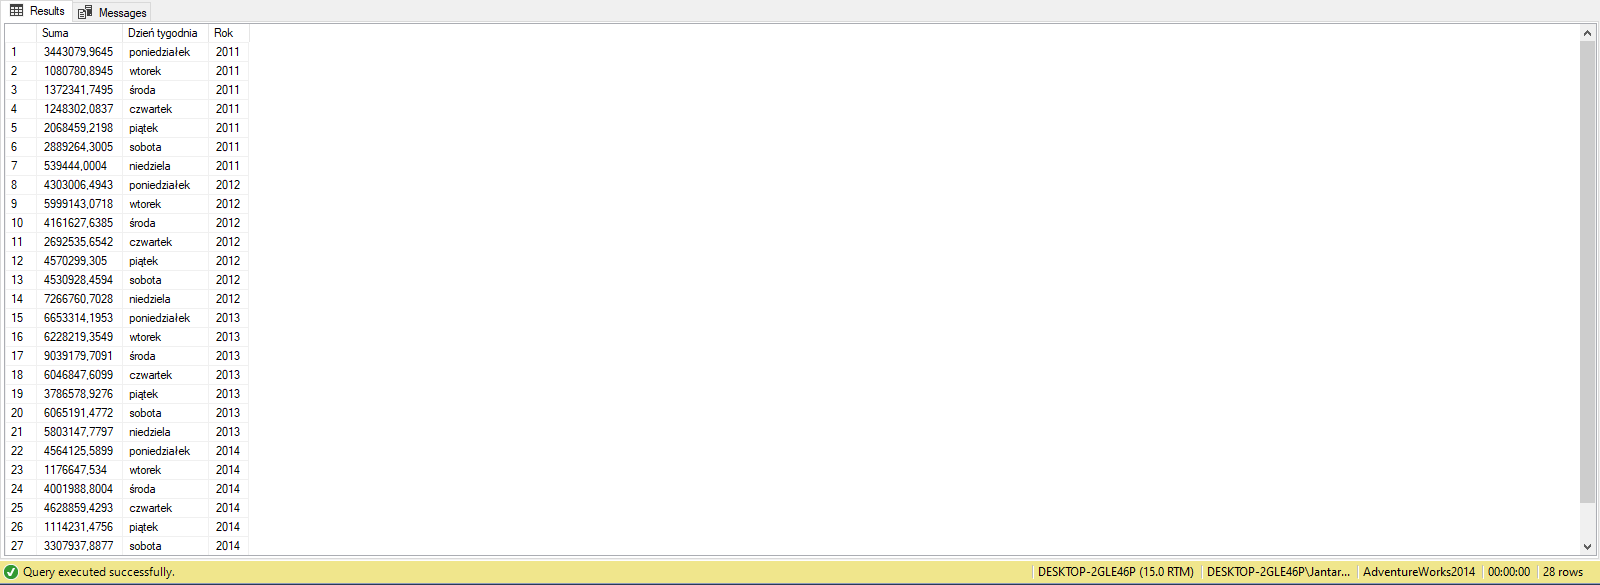
\includegraphics[width=1.0\textwidth]{images/1.png}
  \caption{Wyniki 1. kwerendy}
\end{figure}

W tym podpunkcie użycie CTE nie przyniosłoby korzyści.

\begin{figure}[H]
  \centering
  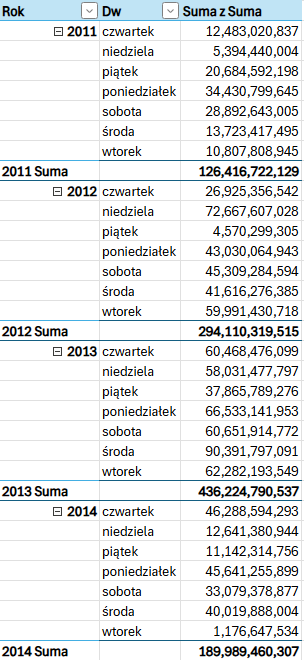
\includegraphics[width=0.4\textwidth]{images/1_excel.png}
  \caption{Tabela przestawna dla 1. kwerendy}
\end{figure}

Dla łatwiejszej analizy dodano tabelę przestawną.

W 2012 i 2013 roku suma roczna szybko rosła. 2014 rok się jeszcze nie skończył, co częściowo wyjaśnia niższą sumę dla 2014 roku.

W 2011 roku przychody w niedzielę były 2 razy niższe niż w drugim najgorszym dniu tygodnia tego roku. Poniedziałek był zdecydowanie najlepszy, a sobota druga.

W 2012 roku piątek był dniem bardzo niskich przychodów - suma była ponad 16 razy mniejsza niż dla najlepszego dnia, niedzieli.

W 2013 roku przychody były bardziej wyrównany, gdzie piątek (najsłabszy dzień) był ponad 2 razy mniej dochodowy niż najlepszy (środa).

W 2014 roku wtorek osiągnął bardzo niski wynik, prawie 40 razy niższy od najlepszego (czwartku).

Wnioskiem jest to, że różne dni w różnych latach odbiegają od normy dla danego roku. Jednak nie w każdym roku różnice były aż tak widoczne.

\end{document}